% !TEX program = xelatex
% !TEX encoding = UTF-8 Unicode
\documentclass{beamer}
\usepackage[no-math]{fontspec}
\usepackage{xeCJK}
\hypersetup{colorlinks,linkcolor=}

\usetheme{CambridgeUS}
\title{Bit-true arithmetics}
\author[jdh8]{何震邦 (Chen-Pang He, jdh8)}
\date{March 19, 2025}
\institute{Skymizer}

\begin{document}
\maketitle

\section{Overview}
\begin{frame}{Overview}
	\tableofcontents
\end{frame}

\begin{frame}{Why}
	\begin{block}{\Huge``}
		\vspace{-1em}
		\begin{enumerate}
			\item The need for an unambiguous specification of the most frequent functions
			\item The only specification that makes sense is correct rounding
			\item Now, correct rounding of many functions is feasible at a very reasonable cost
		\end{enumerate}

		--- Nicolas Brisebarre, Guillaume Hanrot, Jean-Michel Muller, Paul Zimmermann.
		\href
		{https://hal.science/hal-04474530/document}
		{Correctly-rounded evaluation of a function: why, how, and at what cost?}
		2025.  hal-04474530v3
	\end{block}
\end{frame}

\begin{frame}{Quantization}
	\begin{itemize}
		\item Quantization maps a large/continuous set to a small/countable set.
		\item Quantization is required because we only have finite bits to store data.
		\item Further quantization reduces space and probably time usage.
	\end{itemize}
\end{frame}

\begin{frame}{Accuracy and precision}
	\begin{figure}
		\caption{
			\href
			{https://en.wikipedia.org/wiki/Accuracy_and_precision\#ISO_definition_(ISO_5725)}
			{Accuracy according to BIPM and ISO 5725}
		}
		\begin{minipage}{0.4\textwidth}
			\centering
			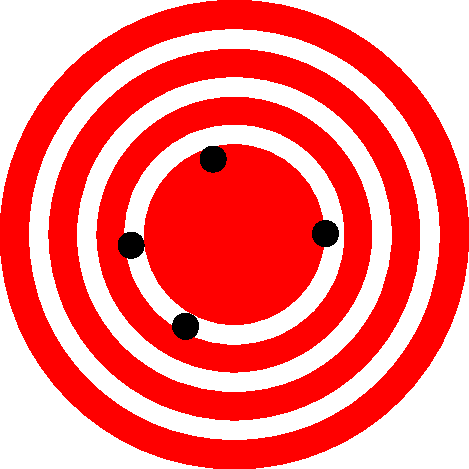
\includegraphics[width=0.8\textwidth]{assets/High_accuracy_Low_precision.pdf} \\
			Low accuracy due to low precision
		\end{minipage}
		\begin{minipage}{0.4\textwidth}
			\centering
			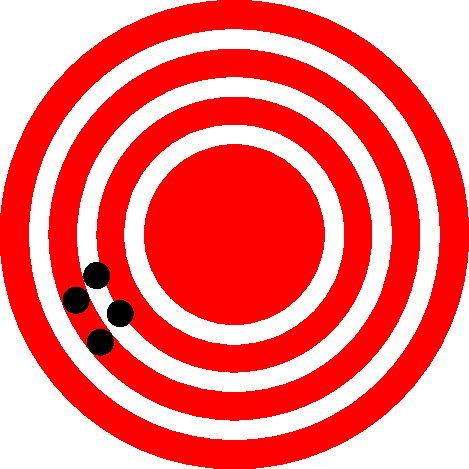
\includegraphics[width=0.8\textwidth]{assets/High_precision_Low_accuracy.pdf} \\
			Low accuracy despite of high precision
		\end{minipage}
	\end{figure}
\end{frame}

\begin{frame}{Rounding modes}
	\begin{figure}
		\href
		{https://upload.wikimedia.org/wikipedia/commons/8/8a/Comparison_rounding_graphs_SMIL.svg}
		{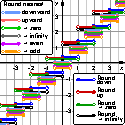
\includegraphics[height=0.625\textheight]{assets/Comparison_rounding_graphs_SMIL.pdf}}

		\caption{
			\href{https://upload.wikimedia.org/wikipedia/commons/8/8a/Comparison_rounding_graphs_SMIL.svg}{Interactive graph}
			by CMG Lee on
			\href{https://commons.wikimedia.org/wiki/File:Comparison_rounding_graphs_SMIL.svg}{Wikimedia Commons}
		}
	\end{figure}
\end{frame}

\section{Algebraic functions}
\begin{frame}{IEEE 754 binary formats}
	\begin{example}
		\begin{figure}
			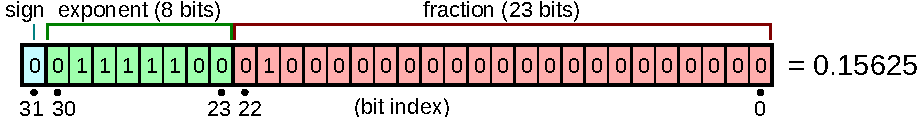
\includegraphics[width=0.8\textwidth]{assets/Float_example.pdf}
			\[ 1.{\color{red}01}_2 \times 2^{{\color{green}124} - 127}  \]
			\begin{center}
				\ttfamily 0x1.{\color{red}4}p{\color{green}-3}
			\end{center}
			\caption{Example normal binary32 by
				\href{https://en.wikipedia.org/wiki/User:Fresheneesz}{Fresheneesz} on
				\href{https://commons.wikimedia.org/wiki/File:Float_example.svg}{Wikipedia}}
		\end{figure}
		\begin{itemize}
			\item (Exponent) bias defaults to $2^{E-1} - 1$.
			\item Implicit bit (1) leads the significand/mantissa.
		\end{itemize}
	\end{example}
\end{frame}

\begin{frame}{Floating-point classification}
	\begin{equation*}
		\begin{cases}
			\text{Infinity | NaN}, & \text{if exponent} = 2^E - 1 \\
			\text{Subnormal | zero}, & \text{if exponent} = 0 \\
			\text{Normal}, & \text{otherwise}
		\end{cases}
	\end{equation*}
\end{frame}

\begin{frame}{Subnormal numbers}
	When the stored exponent is 0,
	\begin{itemize}
		\item The exponent is deemed as 1.
		\item Instead, the implicit bit becomes 0.
	\end{itemize}

	\begin{figure}
		\href
		{https://upload.wikimedia.org/wikipedia/commons/6/69/Denormalized_numbers_on_a_line.svg}
		{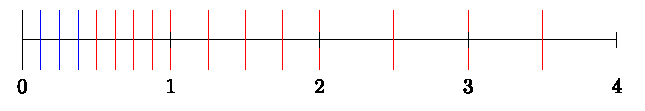
\includegraphics[width=0.8\textwidth]{assets/Denormalized_numbers_on_a_line.pdf}}

		\caption{Seamless transition from 0 to normal numbers by
			\href{https://en.wikipedia.org/wiki/User:Blacklemon67}{Blacklemon67} on
			\href{https://commons.wikimedia.org/wiki/File:Denormalized_numbers_on_a_line.svg}{English Wikipedia}
		}
	\end{figure}
\end{frame}

\begin{frame}{Quiz}
	What is \texttt{std::bit\_cast<float>(0x40000000)}?
\end{frame}

\begin{frame}{Arithmetics}
	Arithmetic results can be inexact in the target format.

	\begin{example}
		Consider 0.1 + 0.2 in IEEE 754 binary64 format.

		\begin{itemize}
			\item 0.1 $\approx$ \texttt{0x1.999999999999ap-4} = \texttt{0x0.6666666666666{\color{red}4}p-2}
			\item 0.2 $\approx$ \texttt{0x1.999999999999ap-3} = \texttt{0x0.ccccccccccccc{\color{red}8}p-2}
			\item 0.3 $\approx$ \texttt{0x1.3333333333333p-2}
		\end{itemize}
		\begin{align*}
			& \textup{binary64}(0.1) + \textup{binary64}(0.2)
			\\ ={}& \texttt{0x1.3333333333333{\color{red}c}p-2}
			\\ \approx{}& \texttt{0x1.3333333333334p-2}
			\\ \approx{}& 0.30000000000000004
		\end{align*}
	\end{example}
\end{frame}

\begin{frame}{Double rounding problem}
	\begin{itemize}
		\item Rounding is not associative!
		\item 9.46 $\to$ 9
		\item 9.46 $\to$ 9.5 $\to$ 10
	\end{itemize}
\end{frame}

\section{Transcendental functions}
\begin{frame}{Table maker's dilemma}
	\begin{itemize}
		\item Let $f =$ target transcendental function.
		\item Let $g =$ algebraic approximation of $f$.
		\item Let $\circ =$ rounding operation.
		\item We cannot prove $\circ f = \circ g$ a priori.
		\item Given any $f \left( x \right) \ne g \left( x \right)$, we cannot
		      be sure if a discontinuity of $\circ$ occurs in between!
	\end{itemize}
\end{frame}

\begin{frame}{\href{https://core-math.gitlabpages.inria.fr/}{CORE-MATH}}
	\begin{itemize}
		\item Correctly rounded in all \href{https://en.cppreference.com/w/c/numeric/fenv/FE_round}{C rounding modes}
		\item Univariate binary32 (\texttt{float}) functions are exhaustively tested.
		\item The rest are tested with known hard-to-round cases.
	\end{itemize}
\end{frame}

\begin{frame}{\href{https://github.com/jdh8/metallic-rs}{\texttt{metallic}}}
	\begin{itemize}
		\item My correctly rounded math library in Rust (WIP)
		\item Correctly rounded in the default rounding mode
		      \begin{itemize}
			      \item Rounding half to even, the only rounding mode in most languages.
			      \item Directed rounding in C/C++ is only guaranteed if
			            \texttt{\#pragma STDC FENV\_ACCESS ON} is set.
		      \end{itemize}
		\item Usually faster than CORE-MATH
	\end{itemize}
\end{frame}

\end{document}